Considérons la fonction homographique $f$ définie sur $\intervalC{0}{- \frac{\beta}{\alpha}}$ par $f(x) = \frac{\alpha x + \beta}{x + \delta}$ où l'on suppose
$\alpha < 0$,
$\beta > 0$
et
$\delta > 0$.%
\footnote{
	Ces contraintes permettent d'obtenir la situation graphique proposée juste après.
}
%
Considérons $M$ un point sur $\setgeo*{C}{f}: y = f(x)$, et le rectangle $MNOP$ comme ci-dessous. Est-il possible de placer $M$ tel que $\area(MNOP)$ soit maximale?

\smallskip

\begin{center}
	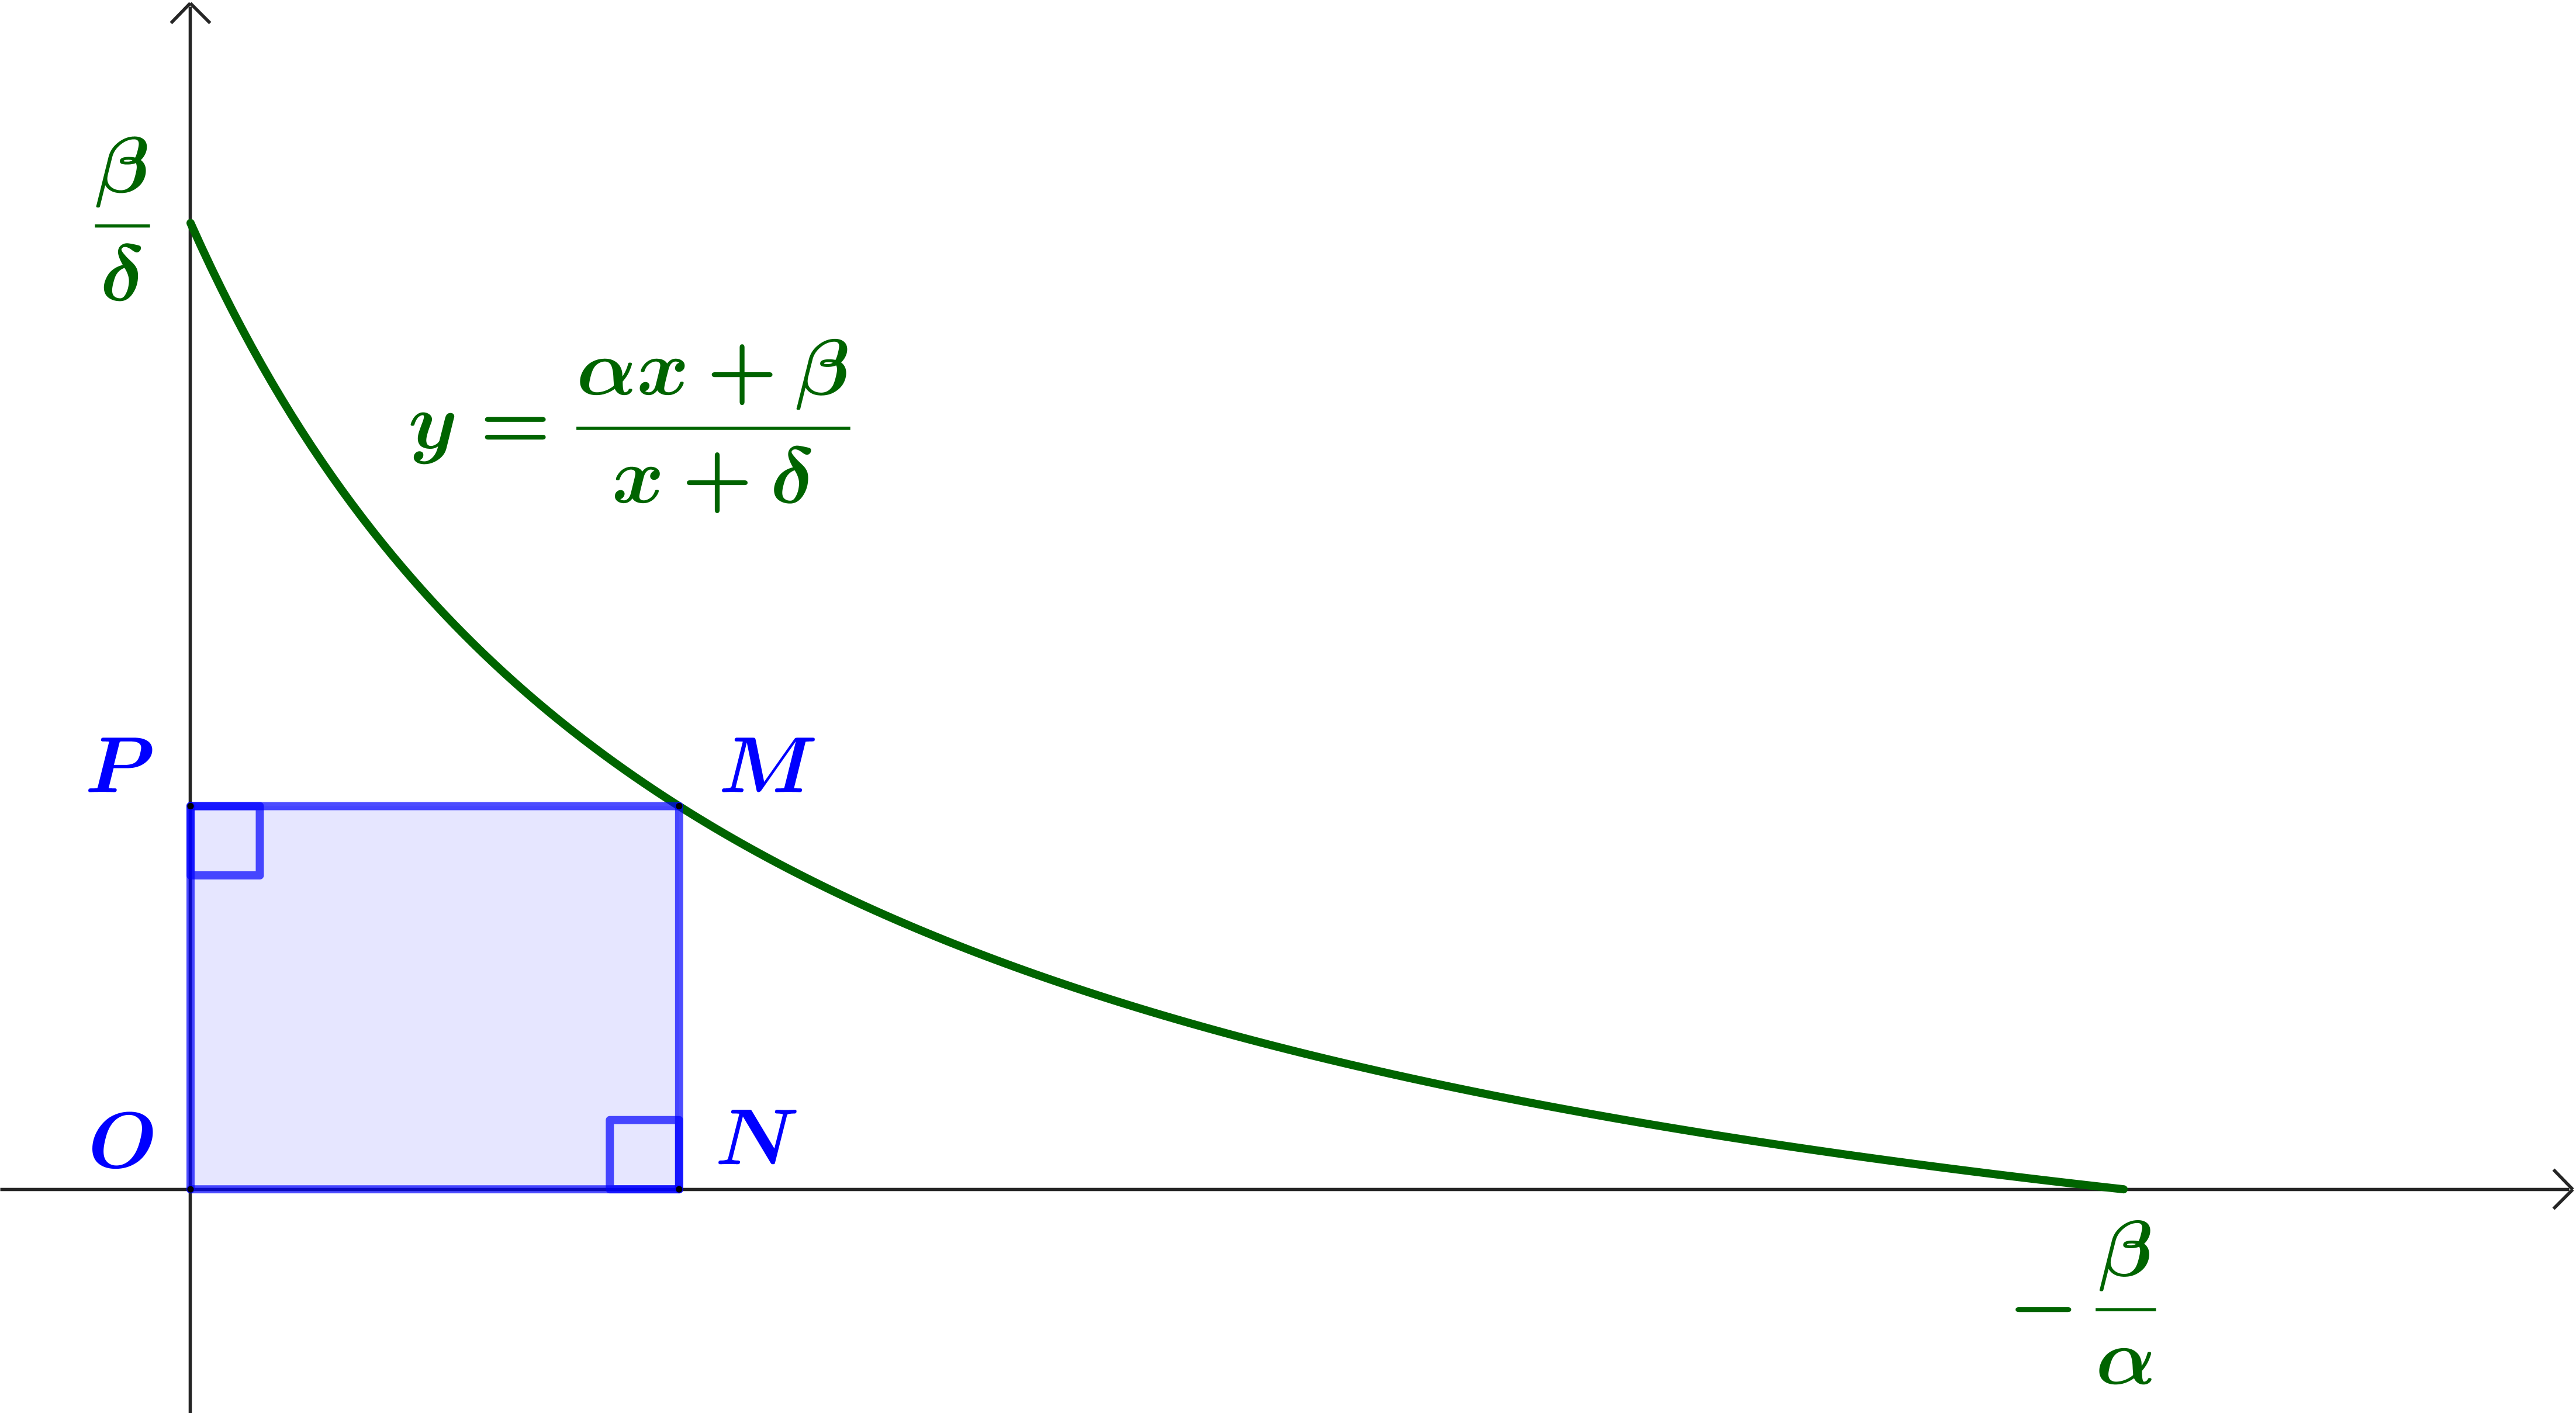
\includegraphics[scale=.67]{goal.png}
\end{center}